\documentclass[a4paper,14pt]{extarticle}

\usepackage[utf8x]{inputenc}
\usepackage[T1,T2A]{fontenc}
\usepackage[russian]{babel}
\usepackage{hyperref}
\usepackage{indentfirst}
\usepackage{here}
\usepackage{array}
\usepackage{graphicx}
\usepackage{caption}
\usepackage{subcaption}
\usepackage{chngcntr}
\usepackage{amsmath}
\usepackage{pgfplots}
\usepackage{pgfplotstable}
\usepackage[left=2cm,right=2cm,top=2cm,bottom=2cm,bindingoffset=0cm]{geometry}

\counterwithin{figure}{section}
\counterwithin{equation}{section}
\counterwithin{table}{section}
\newcommand{\sign}[1][5cm]{\makebox[#1]{\hrulefill}} % Поля подписи и даты
\graphicspath{{pics/}} % Путь до папки с картинками
\captionsetup{justification=centering,margin=1cm}
\def\arraystretch{1.3}

\begin{document}

\begin{titlepage}
\begin{center}
	\textbf{Санкт-Петербургский Политехнический Университет \\Петра Великого}\\[0.3cm]
	\small Институт компьютерных наук и технологий \\[0.3cm]
	\small Кафедра компьютерных систем и программных технологий\\[4cm]
	
	\textbf{ОТЧЕТ}\\ \textbf{о лабораторной работе}\\[0.5cm]
	\textbf{<<Исследование транизисторных ключей>>}\\[0.1cm]
	\textbf{Электротехника и Электроника}\\[10.5cm]
\end{center}

\begin{flushright}
	\begin{minipage}{0.60\textwidth}
		\begin{flushleft}
			\small \textbf{Работу выполнили студенты}\\[3mm]
			\small группа 23501/4 \hspace*{17mm} Дьячков В.В.\\[3mm]
			\small группа 23501/4 \hspace*{17mm} Ламтев А.Ю.\\[5mm]
			
			\small \textbf{Преподаватель}\\[5mm]
		 	\small \sign[3.5cm] \hspace*{8mm} к.т.н., доц. Кочетков Ю.Д.\\[0.5cm]
		\end{flushleft}
	\end{minipage}
\end{flushright}

\vfill

\begin{center}
	\small Санкт-Петербург\\
	\small \the\year
\end{center}
\end{titlepage}

\section{Цель работы}

Исследовать экспериментально переходные процессы, происходящие в транзисторном ключе.

\section{Чертеж схемы исследуемого устройства}

\begin{figure}[H]
\begin{center}
	\vspace{-0.5cm}
	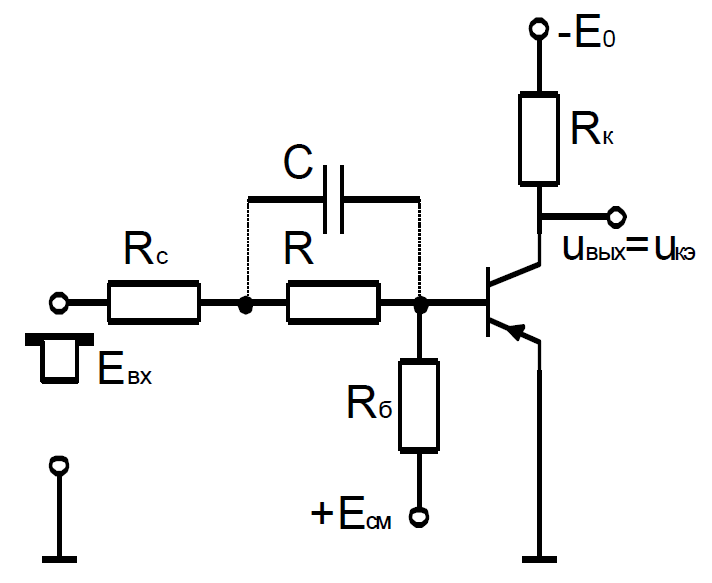
\includegraphics[width=7cm]{scheme}
	\caption{Схема транзисторного ключа с общим эмиттером}
	\vspace{-0.5cm}
\end{center}
\end{figure}

\section{Исходные данные}

Транзистор \verb+МП25+. Германиевый транзистор с $p-n-p$ переходом.

\begin{table}[H]
\begin{center}
	\caption{Исходные данные}
	\def\tabcolsep{12pt}
	\begin{tabular}{|c|c|c|c|c|c|c|c|c|c|}
		\hline
		$E_0$ &
		$E_\text{см}$ &
		$I_\text{кн}$ &
		$S$ &
		$E_\text{вх}$ &
		$t_\text{и}$ &
		$R_c$ &
		$I_{\text{к}_0\ max}$ &
		$B$ &
		$f_\alpha$ \\
		\hline
		В &
		В &
		мА &
		 &
		В &
		мкс &
		кОм &
		мкА &
		 &
		кГц \\
		\hline
		25 &
		5 &
		20 &
		3 &
		7 &
		10 &
		1 &
		75 &
		19 &
		250 \\
	    \hline	
	\end{tabular}
\end{center}
\end{table}

\section{Теоретические расчёты}

\subsection{Расчёт элементов цепи}

\[
R_\text{б} \leq \frac{E_0}{I_{\text{к}_0\ max}} = \frac{25}{75 \cdot 10^{-6}} = 330 \text{ кОм}
\]

\[
R_\text{к} = \frac{E_0}{I_\text{кн}} = \frac{25}{20 \cdot 10^{-3}} = 1.25 \text{ кОм}
\]

\[
I_{\text{б}_1} = \frac{S \cdot I_\text{кн}}{B} = \frac{3 \cdot 20 \cdot 10^{-3}}{19} = 3.16 \text{ мА}
\]

\[
R = \frac{E_\text{вх}}{I_{\text{б}_1} + \frac{E_\text{см}}{R_\text{б}}} - R_\text{c} = \frac{7}{3.16 \cdot 10^{-3} + \frac{5}{330 \cdot 10^3}} - 1 = 1.2 \text{ кОм}
\]

\[
\tau_{\text{б}} = \frac{B}{2 \cdot \pi \cdot f_\alpha} = \frac{19}{2 \cdot \pi \cdot 250 \cdot 10^3} = 1.21 \cdot 10^{-5}
\]

\[
I_{\text{б}_2} \simeq \frac{E_\text{см}}{R_\text{б}} = \frac{5}{330 \cdot 10^3} = 1.51 \cdot 10^{-5} \text{ A}
\]

\[
d = \frac{I_{\text{б}_2}}{I_{\text{б}_1}} = \frac{ 1.51 \cdot 10^{-5}}{3.16 \cdot 10^{-3}} = 4.78 \cdot 10^{-3}
\]

\[
C = \frac{\tau_{\text{б}}}{R \cdot \left( 1 + \frac{dR}{R+R_c} \right)} = \frac{1.21 \cdot 10^{-5}}{1.2 \cdot 10^3 \cdot \left( 1 + \frac{4.78 \cdot 10^{-3} \cdot 1.2 \cdot 10^3}{1.2 \cdot 10^3+1000} \right)} = 10 \text{ нФ}
\]

\subsection{Расчет $t_\text{ф}$, $t_\text{сп}$, $t_\text{расс}$}

\begin{equation}\label{eq:t_f}
t_\phi = \tau_{\text{б}} \cdot \ln{\frac{I_{\text{б}_1}}{I_{\text{б}_1} - 0.9 \cdot \frac{I_\text{кн}}{B}}}
\end{equation}

$I_{\text{б}_2} = 1.51 \cdot 10^{-5} \ll \frac{I_\text{кн}}{B} = \frac{20 \cdot 10^{-3}}{19} \Rightarrow$
\begin{equation}\label{eq:t_sp}
t_\text{сп} = 2.3 \cdot \tau_\text{б}
\end{equation}

$3 \cdot \tau_\text{н} \approx 3 \cdot \tau_{\text{б}} = 3.63 \cdot 10^{-5} \text{ с} > t_\text{и} = 10^{-5} \text{ c} \Rightarrow$

\begin{equation}\label{eq:t_rass}
t_\text{расс} = \tau_{\text{б}} \cdot \ln{\frac{I_{\text{б}_1} \cdot \left( 1 - e^{\frac{-t_\text{и}}{\tau_\text{н}}} \right) + I_{\text{б}_2}}{\frac{I_\text{кн}}{B} + I_{\text{б}_2}}}
\end{equation}

По формулам \ref{eq:t_f}, \ref{eq:t_sp} и \ref{eq:t_rass} найдем $t_\text{ф}$, $t_\text{сп}$ и $t_\text{расс}$ соответственно:

\[
t_\phi = 1.21 \cdot 10^{-5} \cdot \ln{\frac{3.16 \cdot 10^{-3}}{3.16 \cdot 10^{-3} - 0.9 \cdot \frac{20 \cdot 10^{-3}}{19}}} = 4.31 \cdot 10^{-6} \text{ с}
\]
\[
t_\text{сп} = 2.3 \cdot 1.21 \cdot 10^{-5} = 2.78 \cdot 10^{-5} \text{ с}
\]
\[
t_\text{расс} = 1.21 \cdot 10^{-5} \cdot \ln{\frac{3.16 \cdot 10^{-3} \cdot \left( 1 - e^{\frac{-10^{-5}}{1.21 \cdot 10^{-5}}} \right) + 1.51 \cdot 10^{-5}}{\frac{20 \cdot 10^{-3}}{19} + 1.51 \cdot 10^{-5}}} = 6.27 \cdot 10^{-6} \text{ с}
\]

\section{Экспериментально снятые зависимости}

\subsection{Временные диаграммы $U_\text{вх}$, $U_\text{кэ}$ и $U_\text{бэ}$}

На рисунке \ref{fig:time} построены временные диаграммы $U_\text{вх}$, $U_\text{кэ}$ и $U_\text{бэ}$.
	
\begin{figure}[H]
\begin{center}
	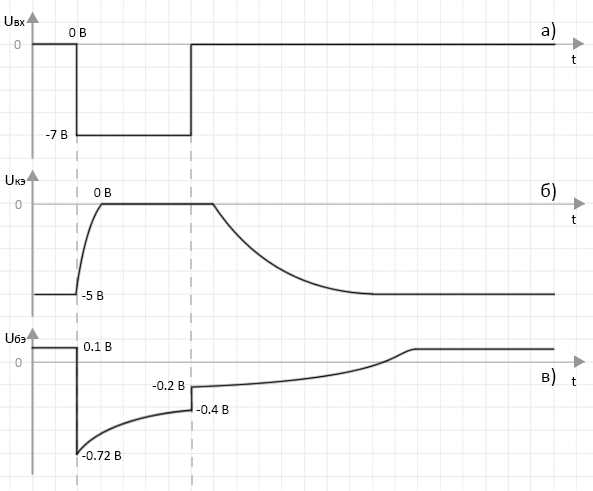
\includegraphics[width=0.9\textwidth]{time}
	\caption{Временные диаграммы: а) $U_\text{вх}$, б) $U_\text{кэ}$, в) $U_\text{бэ}$.}
	\label{fig:time}
\end{center}
\end{figure}

\newpage

\subsection{Зависимость $t_\phi$, $t_\text{сп}$ и $t_\text{расс}$ от $t_\text{и}$}

В таблице \ref{tab:timp} и на рисунке \ref{fig:timp} изображена зависимость $t_\phi$, $t_\text{сп}$ и $t_\text{расс}$ от $t_\text{и}$ ($t_\phi$ и $t_\text{сп}$ не зависят от $t_\text{и}$).

\begin{table}[H]
\begin{center}
	\caption{Зависимость $t_\phi$, $t_\text{сп}$, $t_\text{расс}$ от $t_\text{и}$}
	\label{tab:timp}
	\def\tabcolsep{17pt}
	\pgfplotstabletypeset[col sep=comma,
	    columns={t_i,t_f,t_sp,t_rass},
	    column type/.add={|c|}{},
	    columns/t_i/.style={fixed, column name={$t_\text{и}$, мкс}},
	    columns/t_f/.style={fixed, precision=1, zerofill, column name={$t_\phi$, мкс}},
	    columns/t_sp/.style={fixed, column name={$t_\text{сп}$, мкс}},
	    columns/t_rass/.style={fixed, precision=1, zerofill, column name={$t_\text{расс}$, мкс}},
	    every nth row={1}{before row=\hline},
	    every head row/.style={before row=\hline, after row=\hline},
	    every last row/.style={after row=\hline}
	   ]{data/t_i.csv}
\end{center}
\end{table}

\begin{figure}[H]
\begin{center}
	\begin{tikzpicture} [every plot/.append style={thick}]
		\begin{axis}[
			height=0.35\textheight,
			width=0.75\textwidth,
			legend pos=north west,
			xlabel={$t_\text{и}$, мкс},
			ylabel={$t_\text{расс}$, мкс},
			xlabel near ticks,
			ylabel near ticks,
			xmin = 2,
			xmax = 26,
			ymin = -6,
			ymax = 12,
			grid=major
		]
		\addplot table[x=t_i,y=t_rass,col sep=comma]{data/t_i.csv};
		\addplot table[x=t_i,y=t_rass,col sep=comma]{data/t_i_theory.csv};
		\legend{Эксп., Teор.}
		\end{axis}
	\end{tikzpicture}
	\caption{Зависимость $t_\text{расс}$ от $t_\text{и}$}
	\label{fig:timp}
\end{center}
\end{figure}

\subsection{Зависимость $t_\phi$, $t_\text{сп}$ и $t_\text{расс}$ от $I_{\text{б}_1}$}

В таблице \ref{tab:i_b1} и на рисунке \ref{fig:i_b1} изображена зависимость $t_\phi$, $t_\text{сп}$ и $t_\text{расс}$ от $I_{\text{б}_1}$ ($t_\text{сп}$ не зависит от $I_{\text{б}_1}$).

\begin{table}[H]
\begin{center}
	\caption{Зависимость $t_\phi$, $t_\text{сп}$, $t_\text{расс}$ от $I_{\text{б}_1}$}
	\label{tab:i_b1}
	\def\tabcolsep{17pt}
	\pgfplotstabletypeset[col sep=comma,
	    columns={r,i_b1,t_f,t_sp,t_rass},
	    column type/.add={|c|}{},
	    columns/r/.style={fixed, column name={$R$, Ом}},
	    columns/i_b1/.style={sci, column name={$I_{\text{б}_1}$, А}},
	    columns/t_f/.style={fixed, precision=1, zerofill, column name={$t_\phi$, мкс}},
	    columns/t_sp/.style={fixed, column name={$t_\text{сп}$, мкс}},
	    columns/t_rass/.style={fixed, precision=1, zerofill, column name={$t_\text{расс}$, мкс}},
	    every nth row={1}{before row=\hline},
	    every head row/.style={before row=\hline,after row=\hline},
	    every last row/.style={after row=\hline}
	   ]{data/i_b1.csv}
\end{center}
\end{table}

\begin{figure}[H]
\begin{center}
	\begin{subfigure}[b]{0.45\textwidth}
		\begin{tikzpicture} [every plot/.append style={thick}]
			\begin{axis}[
				height=0.23\textheight,
				width=0.95\textwidth,
				legend pos=north east,
				xlabel={$I_{\text{б}_1}$, А},
				ylabel={$t_\phi$, мкс},
				xlabel near ticks,
				ylabel near ticks,
				grid=major
			]
			\addplot table[x=i_b1,y=t_f,col sep=comma]{data/i_b1.csv};
			\addplot table[x=i_b1,y=t_f,col sep=comma]{data/i_b1_theory.csv};
			\legend{Эксп., Teор.}
			\end{axis}
		\end{tikzpicture}
		\caption{Зависимость $t_\phi$ от $I_{\text{б}_1}$}
	\end{subfigure}
	\begin{subfigure}[b]{0.45\textwidth}
		\begin{tikzpicture} [every plot/.append style={thick}]
			\begin{axis}[
				height=0.23\textheight,
				width=0.95\textwidth,
				legend pos=north west,
				xlabel={$I_{\text{б}_1}$, А},
				ylabel={$t_\text{расс}$, мкс},
				xlabel near ticks,
				ylabel near ticks,
				grid=major
			]
			\addplot table[x=i_b1,y=t_rass,col sep=comma]{data/i_b1.csv};
			\addplot table[x=i_b1,y=t_rass,col sep=comma]{data/i_b1_theory.csv};
			\legend{Эксп., Teор.}
			\end{axis}
		\end{tikzpicture}
		\caption{Зависимость $t_\text{расс}$ от $I_{\text{б}_1}$}
	\end{subfigure}
	\caption{}
	\label{fig:i_b1}
\end{center}
\end{figure}

\newpage

\subsection{Зависимость $t_\phi$, $t_\text{сп}$ и $t_\text{расс}$ от $I_{\text{б}_2}$}

В таблице \ref{tab:i_b2} и на рисунке \ref{fig:i_b2} изображена зависимость $t_\phi$, $t_\text{сп}$ и $t_\text{расс}$ от $I_{\text{б}_2}$ ($t_\phi$ не зависит от $I_{\text{б}_2}$).

\begin{table}[H]
\begin{center}
	\caption{Зависимость $t_\phi$, $t_\text{сп}$, $t_\text{расс}$ от $I_{\text{б}_2}$}
	\label{tab:i_b2}
	\def\tabcolsep{17pt}
	\pgfplotstabletypeset[col sep=comma,
	    columns={r_b,i_b2,t_f,t_sp,t_rass},
	    column type/.add={|c|}{},
	    columns/r_b/.style={fixed, column name={$R_\text{б}$, Ом}},
	    columns/i_b2/.style={sci, column name={$I_{\text{б}_2}$, А}},
	    columns/t_f/.style={fixed, precision=1, zerofill, column name={$t_\phi$, мкс}},
	    columns/t_sp/.style={fixed, column name={$t_\text{сп}$, мкс}},
	    columns/t_rass/.style={fixed, precision=1, zerofill, column name={$t_\text{расс}$, мкс}},
	    every nth row={1}{before row=\hline},
	    every head row/.style={before row=\hline,after row=\hline},
	    every last row/.style={after row=\hline}
	   ]{data/i_b2.csv}
\end{center}
\end{table}

\begin{figure}[H]
\begin{center}
	\begin{subfigure}[b]{0.45\textwidth}
		\begin{tikzpicture} [every plot/.append style={thick}]
			\begin{axis}[
				height=0.23\textheight,
				width=0.95\textwidth,
				legend pos=north east,
				xlabel={$I_{\text{б}_2}$, А},
				ylabel={$t_\text{сп}$, мкс},
				xlabel near ticks,
				ylabel near ticks,
				grid=major
			]
			\addplot table[x=i_b2,y=t_sp,col sep=comma]{data/i_b2.csv};
			\addplot table[x=i_b2,y=t_sp,col sep=comma]{data/i_b2_theory.csv};
			\legend{Эксп., Teор.}
			\end{axis}
		\end{tikzpicture}
		\caption{Зависимость $t_\text{сп}$ от $I_{\text{б}_2}$}
	\end{subfigure}
	\begin{subfigure}[b]{0.45\textwidth}
		\begin{tikzpicture} [every plot/.append style={thick}]
			\begin{axis}[
				height=0.23\textheight,
				width=0.95\textwidth,
				legend pos=north west,
				xlabel={$I_{\text{б}_2}$, А},
				ylabel={$t_\text{расс}$, мкс},
				xlabel near ticks,
				ylabel near ticks,
				ymax=9.5,
				grid=major
			]
			\addplot table[x=i_b2,y=t_rass,col sep=comma]{data/i_b2.csv};
			\addplot table[x=i_b2,y=t_rass,col sep=comma]{data/i_b2_theory.csv};
			\legend{Эксп., Teор.}
			\end{axis}
		\end{tikzpicture}
		\caption{Зависимость $t_\text{расс}$ от $I_{\text{б}_2}$}
	\end{subfigure}
	\caption{}
	\label{fig:i_b2}
\end{center}
\end{figure}

\newpage

\subsection{Зависимость $t_\phi$, $t_\text{сп}$ и $t_\text{расс}$ от $I_{\text{кн}}$}

В таблице \ref{tab:i_kn} и на рисунке \ref{fig:i_kn} изображена зависимость $t_\phi$, $t_\text{сп}$ и $t_\text{расс}$ от $I_{\text{кн}}$ ($t_\phi$ не зависит от $I_{\text{кн}}$).

\begin{table}[H]
\begin{center}
	\caption{Зависимость $t_\phi$, $t_\text{сп}$, $t_\text{расс}$ от $I_{\text{кн}}$}
	\label{tab:i_kn}
	\def\tabcolsep{17pt}
	\pgfplotstabletypeset[col sep=comma,
	    columns={r_k,i_kn,t_f,t_sp,t_rass},
	    column type/.add={|c|}{},
	    columns/r_k/.style={fixed, column name={$R_\text{к}$, Ом}},
	    columns/i_kn/.style={sci, column name={$I_\text{кн}$, А}},
	    columns/t_f/.style={fixed, precision=1, zerofill, column name={$t_\phi$, мкс}},
	    columns/t_sp/.style={fixed, column name={$t_\text{сп}$, мкс}},
	    columns/t_rass/.style={fixed, precision=1, zerofill, column name={$t_\text{расс}$, мкс}},
	    every nth row={1}{before row=\hline},
	    every head row/.style={before row=\hline,after row=\hline},
	    every last row/.style={after row=\hline}
	   ]{data/i_kn.csv}
\end{center}
\end{table}

\vspace{-1cm}

\begin{figure}[H]
\begin{center}
	\begin{subfigure}[b]{0.45\textwidth}
		\begin{tikzpicture} [every plot/.append style={thick}]
			\begin{axis}[
				height=0.23\textheight,
				width=0.95\textwidth,
				legend pos=north west,
				xlabel={$I_\text{кн}$, А},
				ylabel={$t_\phi$, мкс},
				xlabel near ticks,
				ylabel near ticks,
				grid=major
			]
			\addplot table[x=i_kn,y=t_f,col sep=comma]{data/i_kn.csv};
			\addplot table[x=i_kn,y=t_f,col sep=comma]{data/i_kn_theory.csv};
			\legend{Эксп., Teор.}
			\end{axis}
		\end{tikzpicture}
		\caption{Зависимость $t_\phi$ от $I_\text{кн}$}
	\end{subfigure}
	\begin{subfigure}[b]{0.45\textwidth}
		\begin{tikzpicture} [every plot/.append style={thick}]
			\begin{axis}[
				height=0.23\textheight,
				width=0.95\textwidth,
				legend pos=south east,
				xlabel={$I_\text{кн}$, А},
				ylabel={$t_\text{сп}$, мкс},
				xlabel near ticks,
				ylabel near ticks,
				grid=major
			]
			\addplot table[x=i_kn,y=t_sp,col sep=comma]{data/i_kn.csv};
			\addplot table[x=i_kn,y=t_sp,col sep=comma]{data/i_kn_theory.csv};
			\legend{Эксп., Teор.}
			\end{axis}
		\end{tikzpicture}
		\caption{Зависимость $t_\text{сп}$ от $I_\text{кн}$}
	\end{subfigure}\\[0.5cm]
	\begin{subfigure}[b]{0.45\textwidth}
		\begin{tikzpicture} [every plot/.append style={thick}]
			\begin{axis}[
				height=0.23\textheight,
				width=0.95\textwidth,
				legend pos=north east,
				xlabel={$I_\text{кн}$, А},
				ylabel={$t_\text{расс}$, мкс},
				xlabel near ticks,
				ylabel near ticks,
				grid=major
			]
			\addplot table[x=i_kn,y=t_rass,col sep=comma]{data/i_kn.csv};
			\addplot table[x=i_kn,y=t_rass,col sep=comma]{data/i_kn_theory.csv};
			\legend{Эксп., Teор.}
			\end{axis}
		\end{tikzpicture}
		\caption{Зависимость $t_\text{расс}$ от $I_\text{кн}$}
	\end{subfigure}
	\caption{}
	\label{fig:i_kn}
\end{center}
\end{figure}

\subsection{Зависимость $t_\phi$, $t_\text{сп}$ и $t_\text{расс}$ от $C$}

Зашунтировав резистор $R$ конденсатором $C = 10$ нФ, рассчитаем теоретические значения $t_\text{ф}$, $t_\text{сп}$ и $t_\text{расс}$. Для этого в формулы \ref{eq:t_f}, \ref{eq:t_sp} и \ref{eq:t_rass} подставим значение $\tau_\text{б} = \frac{CRR_c}{R+R_c}$:
\[
\tau_\text{б} = \frac{10 \cdot 10^{-9} \cdot 1200 \cdot 1000}{1200 + 1000} = 5.45 \cdot 10^{-6}
\]
\[
t_\phi = 5.45 \cdot 10^{-6} \cdot \ln{\frac{3.16 \cdot 10^{-3}}{3.16 \cdot 10^{-3} - 0.9 \cdot \frac{20 \cdot 10^{-3}}{19}}} = 1.94 \cdot 10^{-6} \text{ с}
\]
\[
t_\text{сп} = 2.3 \cdot 1.21 \cdot 5.45 \cdot 10^{-6} = 6.59 \cdot 10^{-6} \text{ с}
\]
\[
t_\text{расс} = 5.45 \cdot 10^{-6} \cdot \ln{\frac{3.16 \cdot 10^{-3} \cdot \left( 1 - e^{\frac{-10^{-5}}{1.21 \cdot 10^{-5}}} \right) + 1.51 \cdot 10^{-5}}{\frac{20 \cdot 10^{-3}}{19} + 1.51 \cdot 10^{-5}}} = 2.82 \cdot 10^{-6} \text{ с}
\]

В таблице \ref{tab:c} и на рисунке \ref{fig:c} изображена зависимость $t_\phi$, $t_\text{сп}$ и $t_\text{расс}$ от форсирующей емкости $C$.

\begin{table}[H]
\begin{center}
	\caption{Зависимость $t_\phi$, $t_\text{сп}$, $t_\text{расс}$ от $C$}\label{tab:c}
	\def\tabcolsep{17pt}
	\pgfplotstabletypeset[col sep=comma,
	    columns={c,tau_b,t_f,t_sp,t_rass},
	    column type/.add={|c|}{},
	    columns/c/.style={sci, column name={$C$, Ф}},
	    columns/tau_b/.style={sci, column name={$\tau_{\text{б}}$}},
	    columns/t_f/.style={fixed, precision=3, zerofill, column name={$t_\phi$, мкс}},
	    columns/t_sp/.style={fixed, column name={$t_\text{сп}$, мкс}},
	    columns/t_rass/.style={fixed, precision=2, zerofill, column name={$t_\text{расс}$, мкс}},
	    every nth row={1}{before row=\hline},
	    every head row/.style={before row=\hline,after row=\hline},
	    every last row/.style={after row=\hline}
	   ]{data/c.csv}
\end{center}
\end{table}

\begin{figure}[H]
\begin{center}
	\begin{subfigure}[b]{0.45\textwidth}
		\begin{tikzpicture} [every plot/.append style={thick}]
			\begin{axis}[
				height=0.23\textheight,
				width=0.95\textwidth,
				legend pos=north west,
				xlabel={$C$, Ф},
				ylabel={$t_\phi$, мкс},
				xlabel near ticks,
				ylabel near ticks,
				grid=major
			]
			\addplot table[x=c,y=t_f,col sep=comma]{data/c.csv};
			\addplot table[x=c,y=t_f,col sep=comma]{data/c_theory.csv};
			\legend{Эксп., Teор.}
			\end{axis}
		\end{tikzpicture}
		\caption{Зависимость $t_\phi$ от $C$}
	\end{subfigure}
	\begin{subfigure}[b]{0.45\textwidth}
		\begin{tikzpicture} [every plot/.append style={thick}]
			\begin{axis}[
				height=0.23\textheight,
				width=0.95\textwidth,
				legend pos=north west,
				xlabel={$C$, Ф},
				ylabel={$t_\text{сп}$, мкс},
				xlabel near ticks,
				ylabel near ticks,
				grid=major
			]
			\addplot table[x=c,y=t_sp,col sep=comma]{data/c.csv};
			\addplot table[x=c,y=t_sp,col sep=comma]{data/c_theory.csv};
			\legend{Эксп., Teор.}
			\end{axis}
		\end{tikzpicture}
		\caption{Зависимость $t_\text{сп}$ от $C$}
	\end{subfigure}
\end{center}
\end{figure}
\begin{figure}
\begin{center}
\ContinuedFloat
	\begin{subfigure}[b]{0.45\textwidth}
		\begin{tikzpicture} [every plot/.append style={thick}]
			\begin{axis}[
				height=0.23\textheight,
				width=0.95\textwidth,
				legend pos=north west,
				xlabel={$C$, Ф},
				ylabel={$t_\text{расс}$, мкс},
				xlabel near ticks,
				ylabel near ticks,
				grid=major
			]
			\addplot table[x=c,y=t_rass,col sep=comma]{data/c.csv};
			\addplot table[x=c,y=t_rass,col sep=comma]{data/c_theory.csv};
			\legend{Эксп., Teор.}
			\end{axis}
		\end{tikzpicture}
		\caption{Зависимость $t_\text{расс}$ от $C$}
	\end{subfigure}
	\caption{}
	\label{fig:c}
\end{center}
\end{figure}

\section{Выводы}

Полученные экспериментальные зависимости имеют схожий характер изменения с теоретическими. То, что они расположены ниже [на графике], чем теоретические, означает, что реальное значение $f$ транзистора больше, чем указанное в справочнике. 

Таким образом, формулы \ref{eq:t_f}, \ref{eq:t_sp} и \ref{eq:t_rass} являются верными.

\end{document}
